\documentclass{article}\usepackage[]{graphicx}\usepackage[]{xcolor}
% maxwidth is the original width if it is less than linewidth
% otherwise use linewidth (to make sure the graphics do not exceed the margin)
\makeatletter
\def\maxwidth{ %
  \ifdim\Gin@nat@width>\linewidth
    \linewidth
  \else
    \Gin@nat@width
  \fi
}
\makeatother

\definecolor{fgcolor}{rgb}{0.345, 0.345, 0.345}
\newcommand{\hlnum}[1]{\textcolor[rgb]{0.686,0.059,0.569}{#1}}%
\newcommand{\hlstr}[1]{\textcolor[rgb]{0.192,0.494,0.8}{#1}}%
\newcommand{\hlcom}[1]{\textcolor[rgb]{0.678,0.584,0.686}{\textit{#1}}}%
\newcommand{\hlopt}[1]{\textcolor[rgb]{0,0,0}{#1}}%
\newcommand{\hlstd}[1]{\textcolor[rgb]{0.345,0.345,0.345}{#1}}%
\newcommand{\hlkwa}[1]{\textcolor[rgb]{0.161,0.373,0.58}{\textbf{#1}}}%
\newcommand{\hlkwb}[1]{\textcolor[rgb]{0.69,0.353,0.396}{#1}}%
\newcommand{\hlkwc}[1]{\textcolor[rgb]{0.333,0.667,0.333}{#1}}%
\newcommand{\hlkwd}[1]{\textcolor[rgb]{0.737,0.353,0.396}{\textbf{#1}}}%
\let\hlipl\hlkwb

\usepackage{framed}
\makeatletter
\newenvironment{kframe}{%
 \def\at@end@of@kframe{}%
 \ifinner\ifhmode%
  \def\at@end@of@kframe{\end{minipage}}%
  \begin{minipage}{\columnwidth}%
 \fi\fi%
 \def\FrameCommand##1{\hskip\@totalleftmargin \hskip-\fboxsep
 \colorbox{shadecolor}{##1}\hskip-\fboxsep
     % There is no \\@totalrightmargin, so:
     \hskip-\linewidth \hskip-\@totalleftmargin \hskip\columnwidth}%
 \MakeFramed {\advance\hsize-\width
   \@totalleftmargin\z@ \linewidth\hsize
   \@setminipage}}%
 {\par\unskip\endMakeFramed%
 \at@end@of@kframe}
\makeatother

\definecolor{shadecolor}{rgb}{.97, .97, .97}
\definecolor{messagecolor}{rgb}{0, 0, 0}
\definecolor{warningcolor}{rgb}{1, 0, 1}
\definecolor{errorcolor}{rgb}{1, 0, 0}
\newenvironment{knitrout}{}{} % an empty environment to be redefined in TeX

\usepackage{alltt}
\usepackage[sc]{mathpazo}
\renewcommand{\sfdefault}{lmss}
\renewcommand{\ttdefault}{lmtt}
\usepackage[T1]{fontenc}
\usepackage{geometry}
\geometry{verbose,tmargin=2.5cm,bmargin=2.5cm,lmargin=2.5cm,rmargin=2.5cm}
\setcounter{secnumdepth}{2}
\setcounter{tocdepth}{2}
\usepackage[unicode=true,pdfusetitle,
 bookmarks=true,bookmarksnumbered=true,bookmarksopen=true,bookmarksopenlevel=2,
 breaklinks=false,pdfborder={0 0 1},backref=false,colorlinks=false]
 {hyperref}
\hypersetup{
 pdfstartview={XYZ null null 1}}

\makeatletter
%%%%%%%%%%%%%%%%%%%%%%%%%%%%%% User specified LaTeX commands.
\renewcommand{\textfraction}{0.05}
\renewcommand{\topfraction}{0.8}
\renewcommand{\bottomfraction}{0.8}
\renewcommand{\floatpagefraction}{0.75}

\makeatother
\IfFileExists{upquote.sty}{\usepackage{upquote}}{}
\begin{document}



\title{}



\maketitle
The results below are generated from an R script.

\begin{knitrout}
\definecolor{shadecolor}{rgb}{0.969, 0.969, 0.969}\color{fgcolor}\begin{kframe}
\begin{alltt}
\hlcom{# Liberías necesarias para resolver el ejercicio}
\hlkwd{library}\hlstd{(ISLR2)}
\hlkwd{library}\hlstd{(dplyr)}
\hlkwd{library}\hlstd{(caTools)} \hlcom{# Particiones de los datos}
\hlkwd{library}\hlstd{(rpart)} \hlcom{# Para árboles de decisión}
\hlkwd{library}\hlstd{(rpart.plot)}
\hlkwd{library}\hlstd{(ggplot2)}
\hlkwd{library}\hlstd{(caret)} \hlcom{# Para la matriz de confusión}


\hlcom{# Datos}
\hlkwd{attach}\hlstd{(Carseats)}
\end{alltt}


{\ttfamily\noindent\itshape\color{messagecolor}{\#\# The following objects are masked from Carseats (pos = 3):\\\#\# \\\#\# \ \ \ \ Advertising, Age, CompPrice, Education, Income, Population, Price, Sales,\\\#\# \ \ \ \ ShelveLoc, Urban, US}}

{\ttfamily\noindent\itshape\color{messagecolor}{\#\# The following objects are masked from Carseats (pos = 4):\\\#\# \\\#\# \ \ \ \ Advertising, Age, CompPrice, Education, Income, Population, Price, Sales,\\\#\# \ \ \ \ ShelveLoc, Urban, US}}

{\ttfamily\noindent\itshape\color{messagecolor}{\#\# The following objects are masked from Carseats (pos = 8):\\\#\# \\\#\# \ \ \ \ Advertising, Age, CompPrice, Education, Income, Population, Price, Sales,\\\#\# \ \ \ \ ShelveLoc, Urban, US}}\begin{alltt}
\hlcom{# Creamos una nueva variable respuesta binaria}


\hlcom{# Creamos el data frame}

\hlstd{df} \hlkwb{=} \hlstd{Carseats} \hlopt
      \hlkwd{mutate}\hlstd{(}\hlkwc{High} \hlstd{=} \hlkwd{factor}\hlstd{(}\hlkwd{ifelse}\hlstd{(Sales}\hlopt{>=}\hlnum{8}\hlstd{,}\hlstr{"No"}\hlstd{,}\hlstr{"Yes"}\hlstd{)))} \hlopt
      \hlkwd{select}\hlstd{(}\hlopt{-}\hlstd{Sales)}

\hlcom{# Partición de los datos }

\hlcom{# Mediante una semilla conseguimos que el ejercicio sea reproducible}
\hlkwd{set.seed}\hlstd{(}\hlnum{121}\hlstd{)}

\hlcom{# Usamos el 70% de la base de datos como conjunto de entrenamiento y el resto como conjunto de test}
\hlstd{sample} \hlkwb{=} \hlkwd{sample.split}\hlstd{(df}\hlopt{$}\hlstd{High,} \hlkwc{SplitRatio}\hlstd{=}\hlnum{0.7}\hlstd{)}
\hlstd{train}  \hlkwb{=} \hlkwd{subset}\hlstd{(df, sample}\hlopt{==}\hlnum{TRUE}\hlstd{)}
\hlstd{test}   \hlkwb{=} \hlkwd{subset}\hlstd{(df, sample}\hlopt{==}\hlnum{FALSE}\hlstd{)}

\hlcom{# Entrenamos un modelo sobre la muestra de entrenamiento empleando todas las variables}

\hlstd{fit.dt} \hlkwb{=} \hlkwd{rpart}\hlstd{(High}\hlopt{~}\hlstd{.,} \hlkwc{data} \hlstd{= train,} \hlkwc{method} \hlstd{=} \hlstr{'class'}\hlstd{)}
\hlkwd{rpart.plot}\hlstd{(fit.dt,} \hlkwc{extra} \hlstd{=} \hlnum{106}\hlstd{)}
\end{alltt}
\end{kframe}

{\centering 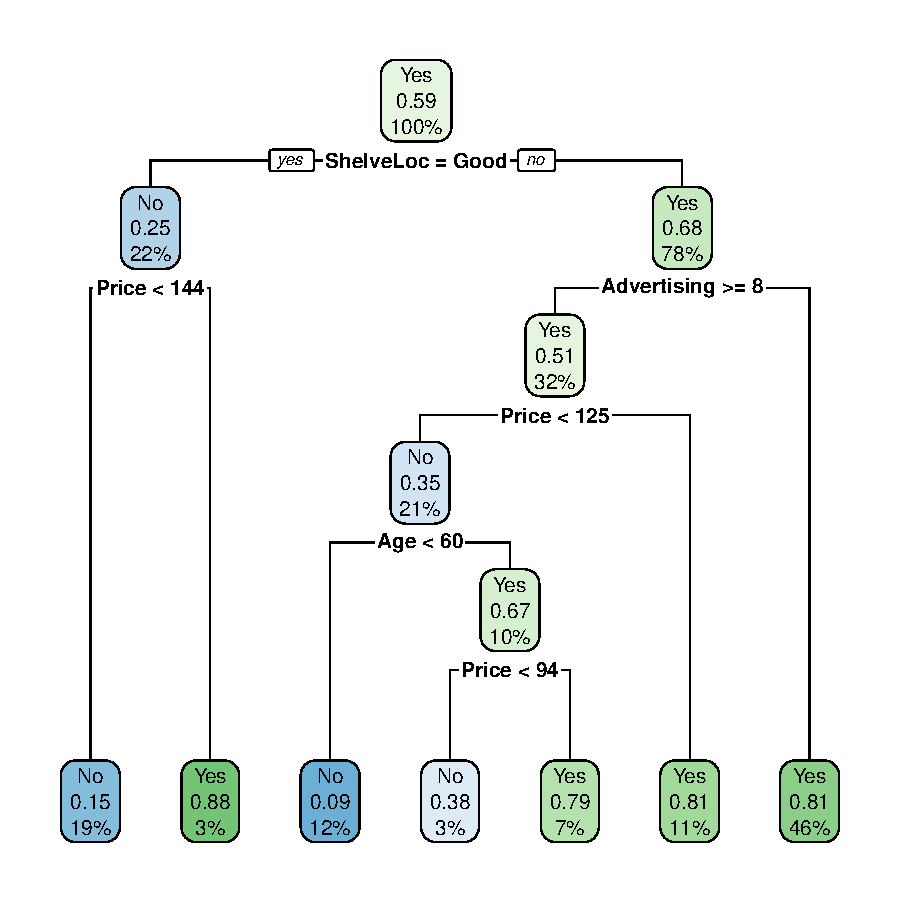
\includegraphics[width=.6\linewidth]{figure/TREE1-SOLUCION-Rnwauto-report-1} 

}


\begin{kframe}\begin{alltt}
\hlcom{# La variable más importante es:}
\hlstd{fit.dt}\hlopt{$}\hlstd{variable.importance}
\end{alltt}
\begin{verbatim}
##   ShelveLoc       Price Advertising         Age   CompPrice          US   Education 
##   19.486155   18.342365   10.575532    9.955631    6.354683    4.737580    2.558957 
##  Population      Income 
##    2.547655    1.973958
\end{verbatim}
\begin{alltt}
\hlcom{# Relación entre la variable respuesta y la variable más importante}
\hlcom{# reordenamos la variable}
\hlstd{train} \hlopt
  \hlkwd{mutate}\hlstd{(}\hlkwc{ShelveLoc_reorder}\hlstd{=}\hlkwd{factor}\hlstd{(ShelveLoc,}\hlkwc{levels}\hlstd{=}\hlkwd{c}\hlstd{(}\hlstr{"Bad"}\hlstd{,}\hlstr{"Medium"}\hlstd{,}\hlstr{"Good"}\hlstd{)))}\hlopt
  \hlkwd{ggplot}\hlstd{(}\hlkwd{aes}\hlstd{(}\hlkwc{x} \hlstd{= ShelveLoc_reorder,} \hlkwc{fill} \hlstd{= High))} \hlopt{+}
  \hlkwd{geom_bar}\hlstd{()}
\end{alltt}
\end{kframe}

{\centering 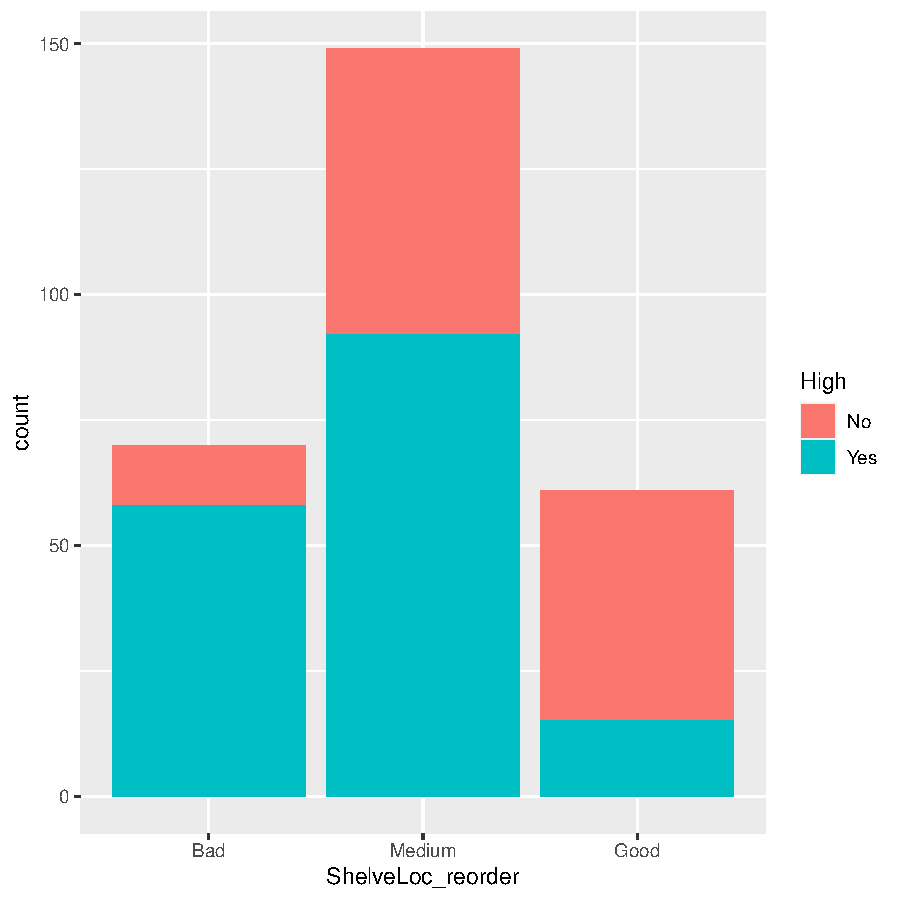
\includegraphics[width=.6\linewidth]{figure/TREE1-SOLUCION-Rnwauto-report-2} 

}


\begin{kframe}\begin{alltt}
\hlcom{# Podemos visualizar su relación con la variable respuesta original como sigue}
\hlcom{# reordenamos la variable}
\hlstd{df} \hlopt
  \hlkwd{mutate}\hlstd{(}\hlkwc{ShelveLoc_reorder}\hlstd{=}\hlkwd{factor}\hlstd{(ShelveLoc,}\hlkwc{levels}\hlstd{=}\hlkwd{c}\hlstd{(}\hlstr{"Bad"}\hlstd{,}\hlstr{"Medium"}\hlstd{,}\hlstr{"Good"}\hlstd{)))}\hlopt
  \hlkwd{ggplot}\hlstd{(}\hlkwd{aes}\hlstd{(ShelveLoc_reorder, Sales))} \hlopt{+}
  \hlkwd{geom_boxplot}\hlstd{()}
\end{alltt}
\end{kframe}

{\centering 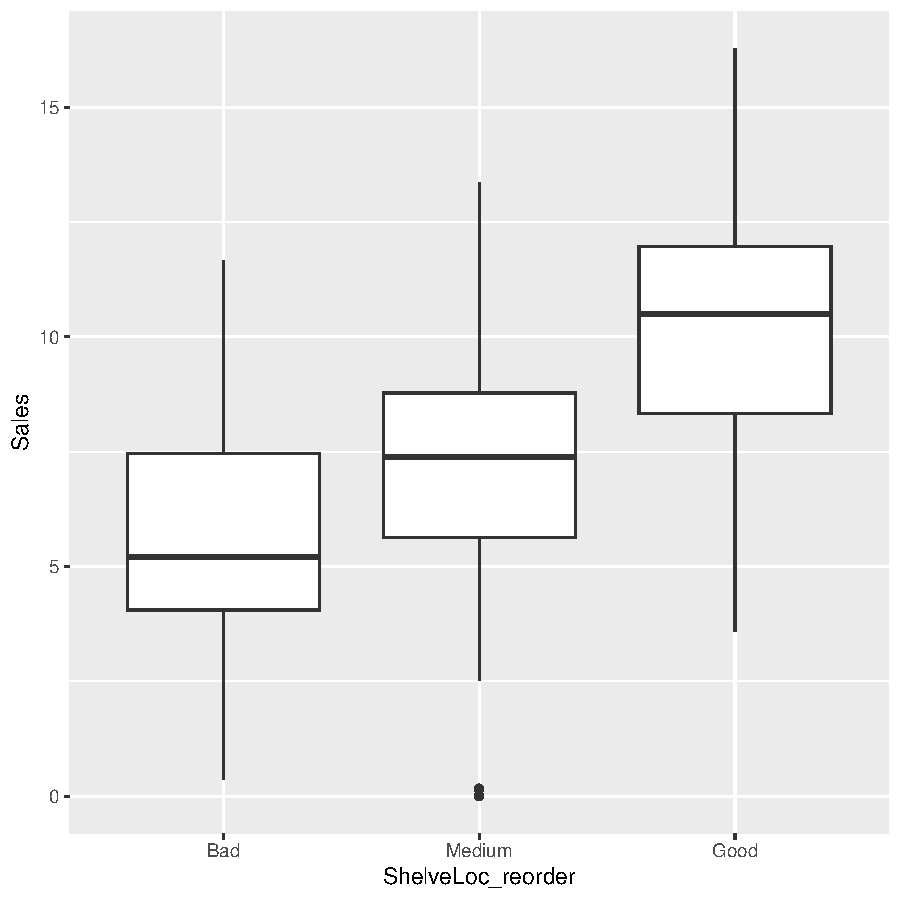
\includegraphics[width=.6\linewidth]{figure/TREE1-SOLUCION-Rnwauto-report-3} 

}


\begin{kframe}\begin{alltt}
\hlcom{# Error de clasificación en train}
\hlcom{# sobre la partición de entrenamiento}
\hlstd{prediction} \hlkwb{=} \hlkwd{predict}\hlstd{(fit.dt, train,} \hlkwc{type} \hlstd{=} \hlstr{'class'}\hlstd{)}
\hlstd{cf} \hlkwb{=} \hlkwd{confusionMatrix}\hlstd{(prediction,} \hlkwd{as.factor}\hlstd{(train}\hlopt{$}\hlstd{High),}\hlkwc{positive}\hlstd{=}\hlstr{"Yes"}\hlstd{)}
\hlkwd{print}\hlstd{(cf)}
\end{alltt}
\begin{verbatim}
## Confusion Matrix and Statistics
## 
##           Reference
## Prediction  No Yes
##        No   80  14
##        Yes  35 151
##                                           
##                Accuracy : 0.825           
##                  95% CI : (0.7753, 0.8676)
##     No Information Rate : 0.5893          
##     P-Value [Acc > NIR] : < 2.2e-16       
##                                           
##                   Kappa : 0.6282          
##                                           
##  Mcnemar's Test P-Value : 0.004275        
##                                           
##             Sensitivity : 0.9152          
##             Specificity : 0.6957          
##          Pos Pred Value : 0.8118          
##          Neg Pred Value : 0.8511          
##              Prevalence : 0.5893          
##          Detection Rate : 0.5393          
##    Detection Prevalence : 0.6643          
##       Balanced Accuracy : 0.8054          
##                                           
##        'Positive' Class : Yes             
## 
\end{verbatim}
\begin{alltt}
\hlcom{# sobre la partición de validación}
\hlstd{prediction} \hlkwb{=} \hlkwd{predict}\hlstd{(fit.dt, test,} \hlkwc{type} \hlstd{=} \hlstr{'class'}\hlstd{)}
\hlstd{cf} \hlkwb{=} \hlkwd{confusionMatrix}\hlstd{(prediction,} \hlkwd{as.factor}\hlstd{(test}\hlopt{$}\hlstd{High),}\hlkwc{positive}\hlstd{=}\hlstr{"Yes"}\hlstd{)}
\hlkwd{print}\hlstd{(cf)}
\end{alltt}
\begin{verbatim}
## Confusion Matrix and Statistics
## 
##           Reference
## Prediction No Yes
##        No  27  10
##        Yes 22  61
##                                           
##                Accuracy : 0.7333          
##                  95% CI : (0.6449, 0.8099)
##     No Information Rate : 0.5917          
##     P-Value [Acc > NIR] : 0.0008589       
##                                           
##                   Kappa : 0.4264          
##                                           
##  Mcnemar's Test P-Value : 0.0518299       
##                                           
##             Sensitivity : 0.8592          
##             Specificity : 0.5510          
##          Pos Pred Value : 0.7349          
##          Neg Pred Value : 0.7297          
##              Prevalence : 0.5917          
##          Detection Rate : 0.5083          
##    Detection Prevalence : 0.6917          
##       Balanced Accuracy : 0.7051          
##                                           
##        'Positive' Class : Yes             
## 
\end{verbatim}
\begin{alltt}
\hlcom{# Ajustamos un modelo con menos profundidad para evitar el sobreajuste.}
\hlstd{control} \hlkwb{=} \hlkwd{rpart.control}\hlstd{(}\hlkwc{minsplit} \hlstd{=} \hlnum{4}\hlstd{,}
                         \hlkwc{minbucket} \hlstd{=} \hlkwd{round}\hlstd{(}\hlnum{5} \hlopt{/} \hlnum{3}\hlstd{),}
                         \hlkwc{maxdepth} \hlstd{=} \hlnum{3}\hlstd{,}
                         \hlkwc{cp} \hlstd{=} \hlnum{0}\hlstd{)}
\hlstd{tune.fit} \hlkwb{=} \hlkwd{rpart}\hlstd{(High}\hlopt{~}\hlstd{.,} \hlkwc{data} \hlstd{= train,} \hlkwc{method} \hlstd{=} \hlstr{'class'}\hlstd{,} \hlkwc{control} \hlstd{= control)}
\hlkwd{rpart.plot}\hlstd{(tune.fit,} \hlkwc{extra} \hlstd{=} \hlnum{106}\hlstd{)}
\end{alltt}
\end{kframe}

{\centering 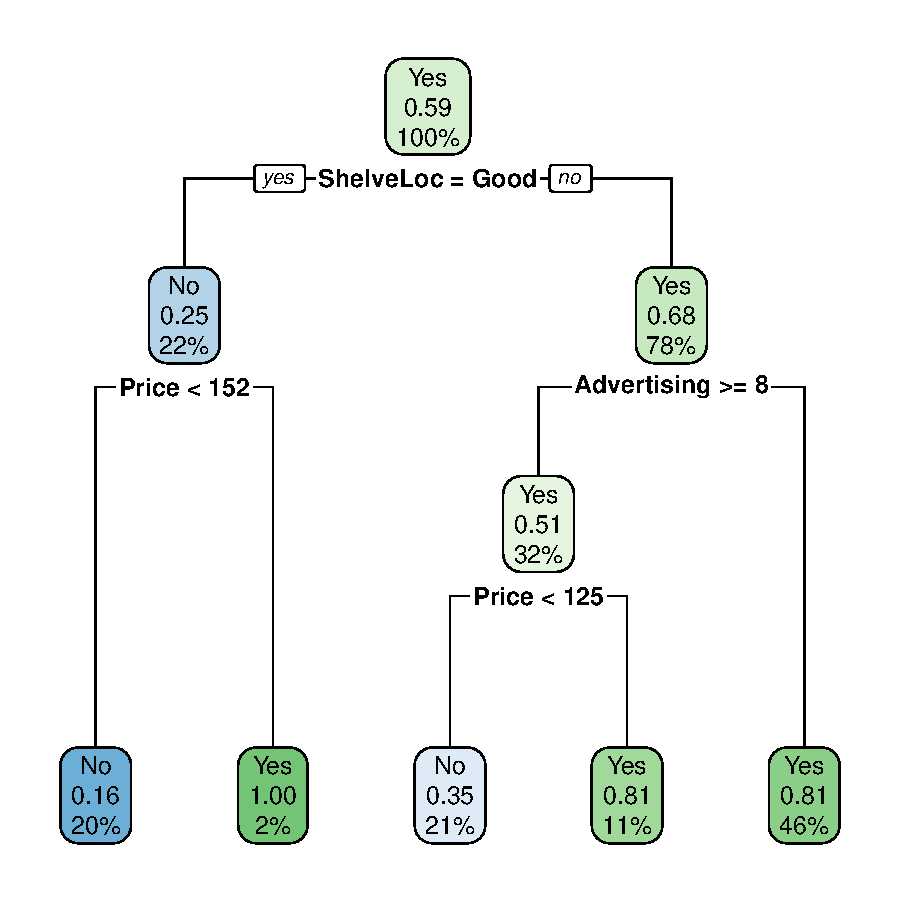
\includegraphics[width=.6\linewidth]{figure/TREE1-SOLUCION-Rnwauto-report-4} 

}


\begin{kframe}\begin{alltt}
\hlcom{# Error de clasificación en train}
\hlcom{# sobre la partición de entrenamiento}
\hlstd{prediction} \hlkwb{=} \hlkwd{predict}\hlstd{(tune.fit, train,} \hlkwc{type} \hlstd{=} \hlstr{'class'}\hlstd{)}
\hlstd{cf} \hlkwb{=} \hlkwd{confusionMatrix}\hlstd{(prediction,} \hlkwd{as.factor}\hlstd{(train}\hlopt{$}\hlstd{High),}\hlkwc{positive}\hlstd{=}\hlstr{"Yes"}\hlstd{)}
\hlkwd{print}\hlstd{(cf)}
\end{alltt}
\begin{verbatim}
## Confusion Matrix and Statistics
## 
##           Reference
## Prediction  No Yes
##        No   85  30
##        Yes  30 135
##                                          
##                Accuracy : 0.7857         
##                  95% CI : (0.733, 0.8323)
##     No Information Rate : 0.5893         
##     P-Value [Acc > NIR] : 2.758e-12      
##                                          
##                   Kappa : 0.5573         
##                                          
##  Mcnemar's Test P-Value : 1              
##                                          
##             Sensitivity : 0.8182         
##             Specificity : 0.7391         
##          Pos Pred Value : 0.8182         
##          Neg Pred Value : 0.7391         
##              Prevalence : 0.5893         
##          Detection Rate : 0.4821         
##    Detection Prevalence : 0.5893         
##       Balanced Accuracy : 0.7787         
##                                          
##        'Positive' Class : Yes            
## 
\end{verbatim}
\begin{alltt}
\hlcom{# sobre la partición de validación}
\hlstd{prediction} \hlkwb{=} \hlkwd{predict}\hlstd{(tune.fit, test,} \hlkwc{type} \hlstd{=} \hlstr{'class'}\hlstd{)}
\hlstd{cf} \hlkwb{=} \hlkwd{confusionMatrix}\hlstd{(prediction,} \hlkwd{as.factor}\hlstd{(test}\hlopt{$}\hlstd{High),}\hlkwc{positive}\hlstd{=}\hlstr{"Yes"}\hlstd{)}
\hlkwd{print}\hlstd{(cf)}
\end{alltt}
\begin{verbatim}
## Confusion Matrix and Statistics
## 
##           Reference
## Prediction No Yes
##        No  32  15
##        Yes 17  56
##                                           
##                Accuracy : 0.7333          
##                  95% CI : (0.6449, 0.8099)
##     No Information Rate : 0.5917          
##     P-Value [Acc > NIR] : 0.0008589       
##                                           
##                   Kappa : 0.4446          
##                                           
##  Mcnemar's Test P-Value : 0.8596838       
##                                           
##             Sensitivity : 0.7887          
##             Specificity : 0.6531          
##          Pos Pred Value : 0.7671          
##          Neg Pred Value : 0.6809          
##              Prevalence : 0.5917          
##          Detection Rate : 0.4667          
##    Detection Prevalence : 0.6083          
##       Balanced Accuracy : 0.7209          
##                                           
##        'Positive' Class : Yes             
## 
\end{verbatim}
\end{kframe}
\end{knitrout}

The R session information (including the OS info, R version and all
packages used):

\begin{knitrout}
\definecolor{shadecolor}{rgb}{0.969, 0.969, 0.969}\color{fgcolor}\begin{kframe}
\begin{alltt}
\hlkwd{sessionInfo}\hlstd{()}
\end{alltt}
\begin{verbatim}
## R version 4.3.1 (2023-06-16)
## Platform: x86_64-pc-linux-gnu (64-bit)
## Running under: Ubuntu 20.04.6 LTS
## 
## Matrix products: default
## BLAS:   /usr/lib/x86_64-linux-gnu/atlas/libblas.so.3.10.3 
## LAPACK: /usr/lib/x86_64-linux-gnu/atlas/liblapack.so.3.10.3;  LAPACK version 3.9.0
## 
## locale:
##  [1] LC_CTYPE=es_ES.UTF-8       LC_NUMERIC=C               LC_TIME=es_ES.UTF-8       
##  [4] LC_COLLATE=es_ES.UTF-8     LC_MONETARY=es_ES.UTF-8    LC_MESSAGES=es_ES.UTF-8   
##  [7] LC_PAPER=es_ES.UTF-8       LC_NAME=C                  LC_ADDRESS=C              
## [10] LC_TELEPHONE=C             LC_MEASUREMENT=es_ES.UTF-8 LC_IDENTIFICATION=C       
## 
## time zone: Europe/Madrid
## tzcode source: system (glibc)
## 
## attached base packages:
## [1] stats     graphics  grDevices utils     datasets  methods   base     
## 
## other attached packages:
## [1] caret_6.0-94     lattice_0.21-9   ggplot2_3.4.3    rpart.plot_3.1.1 rpart_4.1.19    
## [6] caTools_1.18.2   dplyr_1.1.3      ISLR2_1.3-2     
## 
## loaded via a namespace (and not attached):
##  [1] gtable_0.3.4         xfun_0.40            recipes_1.0.8        tzdb_0.4.0          
##  [5] vctrs_0.6.3          tools_4.3.1          bitops_1.0-7         generics_0.1.3      
##  [9] stats4_4.3.1         parallel_4.3.1       proxy_0.4-27         tibble_3.2.1        
## [13] fansi_1.0.5          highr_0.10           ModelMetrics_1.2.2.2 pkgconfig_2.0.3     
## [17] Matrix_1.6-1.1       data.table_1.14.8    lifecycle_1.0.3      stringr_1.5.0       
## [21] compiler_4.3.1       farver_2.1.1         tinytex_0.47         munsell_0.5.0       
## [25] codetools_0.2-19     htmltools_0.5.6.1    class_7.3-22         yaml_2.3.7          
## [29] prodlim_2023.08.28   pillar_1.9.0         MASS_7.3-60          gower_1.0.1         
## [33] iterators_1.0.14     foreach_1.5.2        nlme_3.1-163         parallelly_1.36.0   
## [37] lava_1.7.2.1         tidyselect_1.2.0     digest_0.6.33        stringi_1.7.12      
## [41] future_1.33.0        reshape2_1.4.4       purrr_1.0.2          listenv_0.9.0       
## [45] labeling_0.4.3       splines_4.3.1        fastmap_1.1.1        grid_4.3.1          
## [49] colorspace_2.1-0     cli_3.6.1            magrittr_2.0.3       survival_3.5-7      
## [53] utf8_1.2.3           e1071_1.7-13         future.apply_1.11.0  readr_2.1.4         
## [57] withr_2.5.1          scales_1.2.1         lubridate_1.9.3      timechange_0.2.0    
## [61] rmarkdown_2.25       globals_0.16.2       nnet_7.3-19          timeDate_4022.108   
## [65] hms_1.1.3            evaluate_0.22        knitr_1.44           hardhat_1.3.0       
## [69] rlang_1.1.1          Rcpp_1.0.11          glue_1.6.2           pROC_1.18.4         
## [73] ipred_0.9-14         rstudioapi_0.15.0    R6_2.5.1             plyr_1.8.9
\end{verbatim}
\begin{alltt}
\hlkwd{Sys.time}\hlstd{()}
\end{alltt}
\begin{verbatim}
## [1] "2023-11-01 19:20:14 CET"
\end{verbatim}
\end{kframe}
\end{knitrout}


\end{document}
